\hypertarget{xmlrpc_8inc}{
\section{include/xmlrpc.inc File Reference}
\label{xmlrpc_8inc}\index{include/xmlrpc.inc@{include/xmlrpc.inc}}
}
XML-RPC Library. 

\subsection*{Classes}
\begin{CompactItemize}
\item 
class \hyperlink{classXML}{XML}
\end{CompactItemize}
\subsection*{Functions}
\begin{CompactItemize}
\item 
\& \hyperlink{xmlrpc_8inc_a1e9b05a06f28fabb86c10129f5890ef}{XML\_\-serialize} (\&\$data, \$level=0, \$prior\_\-key=NULL)
\item 
\& \hyperlink{xmlrpc_8inc_ef8f3de498a12b230d049cdee6a25145}{XML\_\-unserialize} (\&\$xml)
\item 
\& \hyperlink{xmlrpc_8inc_708b2136ca600664d2207a511b3cf3f8}{XMLRPC\_\-parse} (\&\$request)
\item 
\& \hyperlink{xmlrpc_8inc_c13be54b26e0803d8745e4f019dcfd8a}{XMLRPC\_\-prepare} (\$data, \$type=NULL)
\item 
\& \hyperlink{xmlrpc_8inc_d936fe41ae9c3e0b90bd72ffe82a2969}{XMLRPC\_\-adjustValue} (\&\$current\_\-node)
\item 
\hyperlink{xmlrpc_8inc_ce4ea8e1274ca2ee3f51ec5a724f00f3}{XMLRPC\_\-getParams} (\$request)
\item 
\hyperlink{xmlrpc_8inc_70efa062e92a380196ed8053850c0906}{XMLRPC\_\-getMethodName} (\$methodCall)
\item 
\hyperlink{xmlrpc_8inc_3a98b6984b8ca01752d1aa9a267526a3}{XMLRPC\_\-request} (\$site, \$location, \$methodName, \$params=NULL, \$user\_\-agent=NULL)
\item 
\hyperlink{xmlrpc_8inc_c736d378caaccdd0726ea1080d1f526f}{XMLRPC\_\-response} (\$return\_\-value, \$server=NULL)
\item 
\hyperlink{xmlrpc_8inc_0cdc54b1376ccbbe412175c9819a95ac}{XMLRPC\_\-error} (\$faultCode, \$faultString, \$server=NULL)
\item 
\hyperlink{xmlrpc_8inc_4485d809c5d598949d9cfaca42bddf37}{XMLRPC\_\-convert\_\-timestamp\_\-to\_\-iso8601} (\$timestamp)
\item 
\hyperlink{xmlrpc_8inc_1d9c2ef61c9f1fd2723d06d1364ef845}{XMLRPC\_\-convert\_\-iso8601\_\-to\_\-timestamp} (\$iso8601)
\item 
\hyperlink{xmlrpc_8inc_88839ba2c5c835c99f55578c65faa401}{count\_\-numeric\_\-items} (\&\$array)
\item 
\hyperlink{xmlrpc_8inc_e2d2e97a8c1c560f5e96d58d60a02874}{XMLRPC\_\-debug} (\$function\_\-name, \$debug\_\-message)
\item 
\hyperlink{xmlrpc_8inc_8467f85edd385ddf2506b1bd5065a6d7}{XMLRPC\_\-debug\_\-print} ()
\item 
\hyperlink{xmlrpc_8inc_1f60d2672bcb35f5ff908f64931f8d48}{XMLRPC\_\-show} (\$data, \$func=\char`\"{}print\_\-r\char`\"{}, \$return\_\-str=false)
\end{CompactItemize}


\subsection{Detailed Description}
XML-RPC Library. 

An XML-RPC implementation by Keith Devens, version 2.5f. \href{http://www.keithdevens.com/software/xmlrpc/}{\tt http://www.keithdevens.com/software/xmlrpc/} Release history available at: \href{http://www.keithdevens.com/software/xmlrpc/history/}{\tt http://www.keithdevens.com/software/xmlrpc/history/} This code is Open Source, released under terms similar to the Artistic License. Read the license at \href{http://www.keithdevens.com/software/license/}{\tt http://www.keithdevens.com/software/license/} Note: this code requires version 4.1.0 or higher of PHP.

\begin{Desc}
\item[See also:]\href{http://keithdevens.com/software/xmlrpc}{\tt http://keithdevens.com/software/xmlrpc}\end{Desc}
\begin{Desc}
\item[\hyperlink{bug__bug000001}{Bug}]Generates the following error on DreamHost servers (and possible others) at different places in the file:\par
 Warning: Call-time pass-by-reference has been deprecated; If you would like to pass it by reference, modify the declaration of xml\_\-set\_\-object(). If you would like to enable call-time pass-by-reference, you can set allow\_\-call\_\-time\_\-pass\_\-reference to true in your INI file. in /home/.zerlina/dkeenan/upc.dankeenan.org/xmlrpc.inc \end{Desc}


Definition in file \hyperlink{xmlrpc_8inc-source}{xmlrpc.inc}.

\subsection{Function Documentation}
\hypertarget{xmlrpc_8inc_88839ba2c5c835c99f55578c65faa401}{
\index{xmlrpc.inc@{xmlrpc.inc}!count_numeric_items@{count\_\-numeric\_\-items}}
\index{count_numeric_items@{count\_\-numeric\_\-items}!xmlrpc.inc@{xmlrpc.inc}}
\subsubsection{\setlength{\rightskip}{0pt plus 5cm}count\_\-numeric\_\-items (\&\$ {\em array})}}
\label{xmlrpc_8inc_88839ba2c5c835c99f55578c65faa401}




Definition at line 473 of file xmlrpc.inc.

Referenced by XML::open(), and XMLRPC\_\-prepare().

\begin{Code}\begin{verbatim}473                                      {
474   return is_array($array) ? count(array_filter(array_keys($array), 'is_numeric')) : 0;
475 }
\end{verbatim}
\end{Code}


\hypertarget{xmlrpc_8inc_a1e9b05a06f28fabb86c10129f5890ef}{
\index{xmlrpc.inc@{xmlrpc.inc}!XML_serialize@{XML\_\-serialize}}
\index{XML_serialize@{XML\_\-serialize}!xmlrpc.inc@{xmlrpc.inc}}
\subsubsection{\setlength{\rightskip}{0pt plus 5cm}\& XML\_\-serialize (\&\$ {\em data}, \$ {\em level} = {\tt 0}, \$ {\em prior\_\-key} = {\tt NULL})}}
\label{xmlrpc_8inc_a1e9b05a06f28fabb86c10129f5890ef}




Definition at line 25 of file xmlrpc.inc.

Referenced by XMLRPC\_\-error(), XMLRPC\_\-request(), and XMLRPC\_\-response().

\begin{Code}\begin{verbatim}25                                                                {
26   #assumes a hash, keys are the variable names
27   $xml_serialized_string = "";
28   while(list($key, $value) = each($data)){
29     $inline = false;
30     $numeric_array = false;
31     $attributes = "";
32     #echo "My current key is '$key', called with prior key '$prior_key'<br>";
33     if(!strstr($key, " attr")){ #if it's not an attribute
34       if(array_key_exists("$key attr", $data)){
35         while(list($attr_name, $attr_value) = each($data["$key attr"])){
36           #echo "Found attribute $attribute_name with value $attribute_value<br>";
37           $attr_value = &htmlspecialchars($attr_value, ENT_QUOTES);
38           $attributes .= " $attr_name=\"$attr_value\"";
39         }
40       }
41 
42       if(is_numeric($key)){
43         #echo "My current key ($key) is numeric. My parent key is '$prior_key'<br>";
44         $key = $prior_key;
45       }else{
46         #you can't have numeric keys at two levels in a row, so this is ok
47         #echo "Checking to see if a numeric key exists in data.";
48         if(is_array($value) and array_key_exists(0, $value)){
49         # echo " It does! Calling myself as a result of a numeric array.<br>";
50           $numeric_array = true;
51           $xml_serialized_string .= XML_serialize($value, $level, $key);
52         }
53         #echo "<br>";
54       }
55 
56       if(!$numeric_array){
57         $xml_serialized_string .= str_repeat("\t", $level) . "<$key$attributes>";
58 
59         if(is_array($value)){
60           $xml_serialized_string .= "\r\n" . XML_serialize($value, $level+1);
61         }else{
62           $inline = true;
63           $xml_serialized_string .= htmlspecialchars($value);
64         }
65 
66         $xml_serialized_string .= (!$inline ? str_repeat("\t", $level) : "") . "</$key>\r\n";
67       }
68     }else{
69       #echo "Skipping attribute record for key $key<bR>";
70     }
71   }
72   if($level == 0){
73     $xml_serialized_string = "<?xml version=\"1.0\" ?>\r\n" . $xml_serialized_string;
74     return $xml_serialized_string;
75   }else{
76     return $xml_serialized_string;
77   }
78 }
\end{verbatim}
\end{Code}


\hypertarget{xmlrpc_8inc_ef8f3de498a12b230d049cdee6a25145}{
\index{xmlrpc.inc@{xmlrpc.inc}!XML_unserialize@{XML\_\-unserialize}}
\index{XML_unserialize@{XML\_\-unserialize}!xmlrpc.inc@{xmlrpc.inc}}
\subsubsection{\setlength{\rightskip}{0pt plus 5cm}\& XML\_\-unserialize (\&\$ {\em xml})}}
\label{xmlrpc_8inc_ef8f3de498a12b230d049cdee6a25145}




Definition at line 167 of file xmlrpc.inc.

Referenced by XMLRPC\_\-parse(), and XMLRPC\_\-request().

\begin{Code}\begin{verbatim}167                                  {
168   $xml_parser = new XML();
169   $data = &$xml_parser->parse(&$xml);
170   $xml_parser->destruct();
171   return $data;
172 }
\end{verbatim}
\end{Code}


\hypertarget{xmlrpc_8inc_d936fe41ae9c3e0b90bd72ffe82a2969}{
\index{xmlrpc.inc@{xmlrpc.inc}!XMLRPC_adjustValue@{XMLRPC\_\-adjustValue}}
\index{XMLRPC_adjustValue@{XMLRPC\_\-adjustValue}!xmlrpc.inc@{xmlrpc.inc}}
\subsubsection{\setlength{\rightskip}{0pt plus 5cm}\& XMLRPC\_\-adjustValue (\&\$ {\em current\_\-node})}}
\label{xmlrpc_8inc_d936fe41ae9c3e0b90bd72ffe82a2969}




Definition at line 245 of file xmlrpc.inc.

Referenced by XMLRPC\_\-getParams(), and XMLRPC\_\-request().

\begin{Code}\begin{verbatim}245                                              {
246   if(is_array($current_node)){
247     if(isset($current_node['array'])){
248       if(!is_array($current_node['array']['data'])){
249         #If there are no elements, return an empty array
250         return array();
251       }else{
252         #echo "Getting rid of array -> data -> value<br>\n";
253         $temp = &$current_node['array']['data']['value'];
254         if(is_array($temp) and array_key_exists(0, $temp)){
255           $count = count($temp);
256           for($n=0;$n<$count;$n++){
257             $temp2[$n] = &XMLRPC_adjustValue(&$temp[$n]);
258           }
259           $temp = &$temp2;
260         }else{
261           $temp2 = &XMLRPC_adjustValue(&$temp);
262           $temp = array(&$temp2);
263           #I do the temp assignment because it avoids copying,
264           # since I can put a reference in the array
265           #PHP's reference model is a bit silly, and I can't just say:
266           # $temp = array(&XMLRPC_adjustValue(&$temp));
267         }
268       }
269     }elseif(isset($current_node['struct'])){
270       if(!is_array($current_node['struct'])){
271         #If there are no members, return an empty array
272         return array();
273       }else{
274         #echo "Getting rid of struct -> member<br>\n";
275         $temp = &$current_node['struct']['member'];
276         if(is_array($temp) and array_key_exists(0, $temp)){
277           $count = count($temp);
278           for($n=0;$n<$count;$n++){
279             #echo "Passing name {$temp[$n][name]}. Value is: " . show($temp[$n][value], var_dump, true) . "<br>\n";
280             $temp2[$temp[$n]['name']] = &XMLRPC_adjustValue(&$temp[$n]['value']);
281             #echo "adjustValue(): After assigning, the value is " . show($temp2[$temp[$n]['name']], var_dump, true) . "<br>\n";
282           }
283         }else{
284           #echo "Passing name $temp[name]<br>\n";
285           $temp2[$temp['name']] = &XMLRPC_adjustValue(&$temp['value']);
286         }
287         $temp = &$temp2;
288       }
289     }else{
290       $types = array('string', 'int', 'i4', 'double', 'dateTime.iso8601', 'base64', 'boolean');
291       $fell_through = true;
292       foreach($types as $type){
293         if(array_key_exists($type, $current_node)){
294           #echo "Getting rid of '$type'<br>\n";
295           $temp = &$current_node[$type];
296           #echo "adjustValue(): The current node is set with a type of $type<br>\n";
297           $fell_through = false;
298           break;
299         }
300       }
301       if($fell_through){
302         $type = 'string';
303         #echo "Fell through! Type is $type<br>\n";
304       }
305       switch ($type){
306         case 'int': case 'i4': $temp = (int)$temp;    break;
307         case 'string':         $temp = (string)$temp; break;
308         case 'double':         $temp = (double)$temp; break;
309         case 'boolean':        $temp = (bool)$temp;   break;
310       }
311     }
312   }else{
313     $temp = (string)$current_node;
314   }
315   return $temp;
316 }
\end{verbatim}
\end{Code}


\hypertarget{xmlrpc_8inc_1d9c2ef61c9f1fd2723d06d1364ef845}{
\index{xmlrpc.inc@{xmlrpc.inc}!XMLRPC_convert_iso8601_to_timestamp@{XMLRPC\_\-convert\_\-iso8601\_\-to\_\-timestamp}}
\index{XMLRPC_convert_iso8601_to_timestamp@{XMLRPC\_\-convert\_\-iso8601\_\-to\_\-timestamp}!xmlrpc.inc@{xmlrpc.inc}}
\subsubsection{\setlength{\rightskip}{0pt plus 5cm}XMLRPC\_\-convert\_\-iso8601\_\-to\_\-timestamp (\$ {\em iso8601})}}
\label{xmlrpc_8inc_1d9c2ef61c9f1fd2723d06d1364ef845}




Definition at line 469 of file xmlrpc.inc.

\begin{Code}\begin{verbatim}469                                                       {
470   return strtotime($iso8601);
471 }
\end{verbatim}
\end{Code}


\hypertarget{xmlrpc_8inc_4485d809c5d598949d9cfaca42bddf37}{
\index{xmlrpc.inc@{xmlrpc.inc}!XMLRPC_convert_timestamp_to_iso8601@{XMLRPC\_\-convert\_\-timestamp\_\-to\_\-iso8601}}
\index{XMLRPC_convert_timestamp_to_iso8601@{XMLRPC\_\-convert\_\-timestamp\_\-to\_\-iso8601}!xmlrpc.inc@{xmlrpc.inc}}
\subsubsection{\setlength{\rightskip}{0pt plus 5cm}XMLRPC\_\-convert\_\-timestamp\_\-to\_\-iso8601 (\$ {\em timestamp})}}
\label{xmlrpc_8inc_4485d809c5d598949d9cfaca42bddf37}




Definition at line 463 of file xmlrpc.inc.

\begin{Code}\begin{verbatim}463                                                         {
464   #takes a unix timestamp and converts it to iso8601 required by XMLRPC
465   #an example iso8601 datetime is "20010822T03:14:33"
466   return date("Ymd\TH:i:s", $timestamp);
467 }
\end{verbatim}
\end{Code}


\hypertarget{xmlrpc_8inc_e2d2e97a8c1c560f5e96d58d60a02874}{
\index{xmlrpc.inc@{xmlrpc.inc}!XMLRPC_debug@{XMLRPC\_\-debug}}
\index{XMLRPC_debug@{XMLRPC\_\-debug}!xmlrpc.inc@{xmlrpc.inc}}
\subsubsection{\setlength{\rightskip}{0pt plus 5cm}XMLRPC\_\-debug (\$ {\em function\_\-name}, \$ {\em debug\_\-message})}}
\label{xmlrpc_8inc_e2d2e97a8c1c560f5e96d58d60a02874}




Definition at line 477 of file xmlrpc.inc.

Referenced by XMLRPC\_\-error(), XMLRPC\_\-parse(), XMLRPC\_\-request(), and XMLRPC\_\-response().

\begin{Code}\begin{verbatim}477                                                      {
478   $GLOBALS['XMLRPC_DEBUG_INFO'][] = array($function_name, $debug_message);
479 }
\end{verbatim}
\end{Code}


\hypertarget{xmlrpc_8inc_8467f85edd385ddf2506b1bd5065a6d7}{
\index{xmlrpc.inc@{xmlrpc.inc}!XMLRPC_debug_print@{XMLRPC\_\-debug\_\-print}}
\index{XMLRPC_debug_print@{XMLRPC\_\-debug\_\-print}!xmlrpc.inc@{xmlrpc.inc}}
\subsubsection{\setlength{\rightskip}{0pt plus 5cm}XMLRPC\_\-debug\_\-print ()}}
\label{xmlrpc_8inc_8467f85edd385ddf2506b1bd5065a6d7}




Definition at line 481 of file xmlrpc.inc.

References \$debug.

\begin{Code}\begin{verbatim}481                              {
482   if($GLOBALS['XMLRPC_DEBUG_INFO']){
483     echo "<table border=\"1\" width=\"100%\">\n";
484     foreach($GLOBALS['XMLRPC_DEBUG_INFO'] as $debug){
485       echo "<tr><th style=\"vertical-align: top\">$debug[0]</th><td>$debug[1]</td></tr>\n";
486     }
487     echo "</table>\n";
488     unset($GLOBALS['XMLRPC_DEBUG_INFO']);
489   }else{
490     echo "<p>No debugging information available yet.</p>";
491   }
492 }
\end{verbatim}
\end{Code}


\hypertarget{xmlrpc_8inc_0cdc54b1376ccbbe412175c9819a95ac}{
\index{xmlrpc.inc@{xmlrpc.inc}!XMLRPC_error@{XMLRPC\_\-error}}
\index{XMLRPC_error@{XMLRPC\_\-error}!xmlrpc.inc@{xmlrpc.inc}}
\subsubsection{\setlength{\rightskip}{0pt plus 5cm}XMLRPC\_\-error (\$ {\em faultCode}, \$ {\em faultString}, \$ {\em server} = {\tt NULL})}}
\label{xmlrpc_8inc_0cdc54b1376ccbbe412175c9819a95ac}




Definition at line 440 of file xmlrpc.inc.

References XML\_\-serialize(), XMLRPC\_\-debug(), and XMLRPC\_\-show().

\begin{Code}\begin{verbatim}440                                                                {
441   $array["methodResponse"]["fault"]["value"]["struct"]["member"] = array();
442   $temp = &$array["methodResponse"]["fault"]["value"]["struct"]["member"];
443   $temp[0]["name"] = "faultCode";
444   $temp[0]["value"]["int"] = $faultCode;
445   $temp[1]["name"] = "faultString";
446   $temp[1]["value"]["string"] = $faultString;
447 
448   $return = XML_serialize($array);
449 
450   header("Connection: close");
451   header("Content-Length: " . strlen($return));
452   header("Content-Type: text/xml");
453   header("Date: " . date("r"));
454   if($server){
455     header("Server: $server");
456   }
457   if(defined('XMLRPC_DEBUG') and XMLRPC_DEBUG){
458     XMLRPC_debug('XMLRPC_error', "<p>Sent the following error response:</p>\n\n" . XMLRPC_show($return, 'print_r', true));
459   }
460   echo $return;
461 }
\end{verbatim}
\end{Code}




Here is the call graph for this function:\nopagebreak
\begin{figure}[H]
\begin{center}
\leavevmode
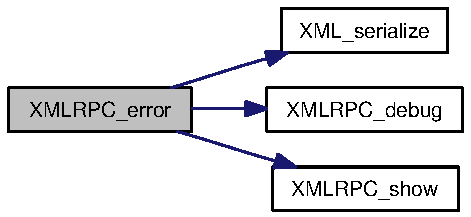
\includegraphics[width=131pt]{xmlrpc_8inc_0cdc54b1376ccbbe412175c9819a95ac_cgraph}
\end{center}
\end{figure}
\hypertarget{xmlrpc_8inc_70efa062e92a380196ed8053850c0906}{
\index{xmlrpc.inc@{xmlrpc.inc}!XMLRPC_getMethodName@{XMLRPC\_\-getMethodName}}
\index{XMLRPC_getMethodName@{XMLRPC\_\-getMethodName}!xmlrpc.inc@{xmlrpc.inc}}
\subsubsection{\setlength{\rightskip}{0pt plus 5cm}XMLRPC\_\-getMethodName (\$ {\em methodCall})}}
\label{xmlrpc_8inc_70efa062e92a380196ed8053850c0906}




Definition at line 339 of file xmlrpc.inc.

\begin{Code}\begin{verbatim}339                                           {
340   #returns the method name
341   return $methodCall['methodCall']['methodName'];
342 }
\end{verbatim}
\end{Code}


\hypertarget{xmlrpc_8inc_ce4ea8e1274ca2ee3f51ec5a724f00f3}{
\index{xmlrpc.inc@{xmlrpc.inc}!XMLRPC_getParams@{XMLRPC\_\-getParams}}
\index{XMLRPC_getParams@{XMLRPC\_\-getParams}!xmlrpc.inc@{xmlrpc.inc}}
\subsubsection{\setlength{\rightskip}{0pt plus 5cm}XMLRPC\_\-getParams (\$ {\em request})}}
\label{xmlrpc_8inc_ce4ea8e1274ca2ee3f51ec5a724f00f3}




Definition at line 318 of file xmlrpc.inc.

References XMLRPC\_\-adjustValue().

\begin{Code}\begin{verbatim}318                                    {
319   if(!is_array($request['methodCall']['params'])){
320     #If there are no parameters, return an empty array
321     return array();
322   }else{
323     #echo "Getting rid of methodCall -> params -> param<br>\n";
324     $temp = &$request['methodCall']['params']['param'];
325     if(is_array($temp) and array_key_exists(0, $temp)){
326       $count = count($temp);
327       for($n = 0; $n < $count; $n++){
328         #echo "Serializing parameter $n<br>";
329         $temp2[$n] = &XMLRPC_adjustValue(&$temp[$n]['value']);
330       }
331     }else{
332       $temp2[0] = &XMLRPC_adjustValue($temp['value']);
333     }
334     $temp = &$temp2;
335     return $temp;
336   }
337 }
\end{verbatim}
\end{Code}




Here is the call graph for this function:\nopagebreak
\begin{figure}[H]
\begin{center}
\leavevmode
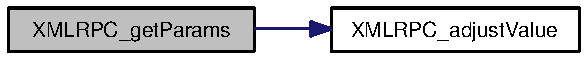
\includegraphics[width=159pt]{xmlrpc_8inc_ce4ea8e1274ca2ee3f51ec5a724f00f3_cgraph}
\end{center}
\end{figure}
\hypertarget{xmlrpc_8inc_708b2136ca600664d2207a511b3cf3f8}{
\index{xmlrpc.inc@{xmlrpc.inc}!XMLRPC_parse@{XMLRPC\_\-parse}}
\index{XMLRPC_parse@{XMLRPC\_\-parse}!xmlrpc.inc@{xmlrpc.inc}}
\subsubsection{\setlength{\rightskip}{0pt plus 5cm}\& XMLRPC\_\-parse (\&\$ {\em request})}}
\label{xmlrpc_8inc_708b2136ca600664d2207a511b3cf3f8}




Definition at line 174 of file xmlrpc.inc.

References XML\_\-unserialize(), XMLRPC\_\-debug(), and XMLRPC\_\-show().

\begin{Code}\begin{verbatim}174                                   {
175   if(defined('XMLRPC_DEBUG') and XMLRPC_DEBUG){
176     XMLRPC_debug('XMLRPC_parse', "<p>Received the following raw request:</p>" . XMLRPC_show($request, 'print_r', true));
177   }
178   $data = &XML_unserialize(&$request);
179   if(defined('XMLRPC_DEBUG') and XMLRPC_DEBUG){
180     XMLRPC_debug('XMLRPC_parse', "<p>Returning the following parsed request:</p>" . XMLRPC_show($data, 'print_r', true));
181   }
182   return $data;
183 }
\end{verbatim}
\end{Code}




Here is the call graph for this function:\nopagebreak
\begin{figure}[H]
\begin{center}
\leavevmode
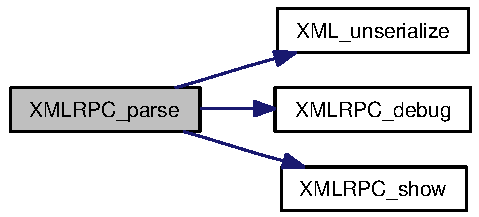
\includegraphics[width=133pt]{xmlrpc_8inc_708b2136ca600664d2207a511b3cf3f8_cgraph}
\end{center}
\end{figure}
\hypertarget{xmlrpc_8inc_c13be54b26e0803d8745e4f019dcfd8a}{
\index{xmlrpc.inc@{xmlrpc.inc}!XMLRPC_prepare@{XMLRPC\_\-prepare}}
\index{XMLRPC_prepare@{XMLRPC\_\-prepare}!xmlrpc.inc@{xmlrpc.inc}}
\subsubsection{\setlength{\rightskip}{0pt plus 5cm}\& XMLRPC\_\-prepare (\$ {\em data}, \$ {\em type} = {\tt NULL})}}
\label{xmlrpc_8inc_c13be54b26e0803d8745e4f019dcfd8a}




Definition at line 185 of file xmlrpc.inc.

References count\_\-numeric\_\-items().

Referenced by checkBarcode(), and getBarcodeInfo().

\begin{Code}\begin{verbatim}185                                               {
186   if(is_array($data)){
187     $num_elements = count($data);
188     if((array_key_exists(0, $data) or !$num_elements) and $type != 'struct'){ #it's an array
189       if(!$num_elements){ #if the array is empty
190         $returnvalue =  array('array' => array('data' => NULL));
191       }else{
192         $returnvalue['array']['data']['value'] = array();
193         $temp = &$returnvalue['array']['data']['value'];
194         $count = count_numeric_items($data);
195         for($n=0; $n<$count; $n++){
196           $type = NULL;
197           if(array_key_exists("$n type", $data)){
198             $type = $data["$n type"];
199           }
200           $temp[$n] = XMLRPC_prepare(&$data[$n], $type);
201         }
202       }
203     }else{ #it's a struct
204       if(!$num_elements){ #if the struct is empty
205         $returnvalue = array('struct' => NULL);
206       }else{
207         $returnvalue['struct']['member'] = array();
208         $temp = &$returnvalue['struct']['member'];
209         while(list($key, $value) = each($data)){
210           if(substr($key, -5) != ' type'){ #if it's not a type specifier
211             $type = NULL;
212             if(array_key_exists("$key type", $data)){
213               $type = $data["$key type"];
214             }
215             $temp[] = array('name' => $key, 'value' => XMLRPC_prepare(&$value, $type));
216           }
217         }
218       }
219     }
220   }else{ #it's a scalar
221     if(!$type){
222       if(is_int($data)){
223         $returnvalue['int'] = $data;
224         return $returnvalue;
225       }elseif(is_float($data)){
226         $returnvalue['double'] = $data;
227         return $returnvalue;
228       }elseif(is_bool($data)){
229         $returnvalue['boolean'] = ($data ? 1 : 0);
230         return $returnvalue;
231       }elseif(preg_match('/^\d{8}T\d{2}:\d{2}:\d{2}$/', $data, $matches)){ #it's a date
232         $returnvalue['dateTime.iso8601'] = $data;
233         return $returnvalue;
234       }elseif(is_string($data)){
235         $returnvalue['string'] = htmlspecialchars($data);
236         return $returnvalue;
237       }
238     }else{
239       $returnvalue[$type] = htmlspecialchars($data);
240     }
241   }
242   return $returnvalue;
243 }
\end{verbatim}
\end{Code}




Here is the call graph for this function:\nopagebreak
\begin{figure}[H]
\begin{center}
\leavevmode
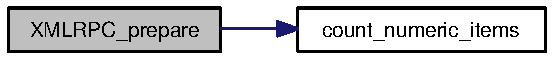
\includegraphics[width=151pt]{xmlrpc_8inc_c13be54b26e0803d8745e4f019dcfd8a_cgraph}
\end{center}
\end{figure}
\hypertarget{xmlrpc_8inc_3a98b6984b8ca01752d1aa9a267526a3}{
\index{xmlrpc.inc@{xmlrpc.inc}!XMLRPC_request@{XMLRPC\_\-request}}
\index{XMLRPC_request@{XMLRPC\_\-request}!xmlrpc.inc@{xmlrpc.inc}}
\subsubsection{\setlength{\rightskip}{0pt plus 5cm}XMLRPC\_\-request (\$ {\em site}, \$ {\em location}, \$ {\em methodName}, \$ {\em params} = {\tt NULL}, \$ {\em user\_\-agent} = {\tt NULL})}}
\label{xmlrpc_8inc_3a98b6984b8ca01752d1aa9a267526a3}




Definition at line 344 of file xmlrpc.inc.

References XML\_\-serialize(), XML\_\-unserialize(), XMLRPC\_\-adjustValue(), XMLRPC\_\-debug(), and XMLRPC\_\-show().

Referenced by checkBarcode(), and getBarcodeInfo().

\begin{Code}\begin{verbatim}344                                                                                           {
345   $site = explode(':', $site);
346   if(isset($site[1]) and is_numeric($site[1])){
347     $port = $site[1];
348   }else{
349     $port = 80;
350   }
351   $site = $site[0];
352 
353   $data["methodCall"]["methodName"] = $methodName;
354   $param_count = count($params);
355   if(!$param_count){
356     $data["methodCall"]["params"] = NULL;
357   }else{
358     for($n = 0; $n<$param_count; $n++){
359       $data["methodCall"]["params"]["param"][$n]["value"] = $params[$n];
360     }
361   }
362   $data = XML_serialize($data);
363 
364   if(defined('XMLRPC_DEBUG') and XMLRPC_DEBUG){
365     XMLRPC_debug('XMLRPC_request', "<p>Received the following parameter list to send:</p>" . XMLRPC_show($params, 'print_r', true));
366   }
367   $conn = fsockopen ($site, $port); #open the connection
368   if(!$conn){ #if the connection was not opened successfully
369     if(defined('XMLRPC_DEBUG') and XMLRPC_DEBUG){
370       XMLRPC_debug('XMLRPC_request', "<p>Connection failed: Couldn't make the connection to $site.</p>");
371     }
372     return array(false, array('faultCode'=>10532, 'faultString'=>"Connection failed: Couldn't make the connection to $site."));
373   }else{
374     $headers =
375       "POST $location HTTP/1.0\r\n" .
376       "Host: $site\r\n" .
377       "Connection: close\r\n" .
378       ($user_agent ? "User-Agent: $user_agent\r\n" : '') .
379       "Content-Type: text/xml\r\n" .
380       "Content-Length: " . strlen($data) . "\r\n\r\n";
381 
382     fputs($conn, "$headers");
383     fputs($conn, $data);
384 
385     if(defined('XMLRPC_DEBUG') and XMLRPC_DEBUG){
386       XMLRPC_debug('XMLRPC_request', "<p>Sent the following request:</p>\n\n" . XMLRPC_show($headers . $data, 'print_r', true));
387     }
388 
389     #socket_set_blocking ($conn, false);
390     $response = "";
391     while(!feof($conn)){
392       $response .= fgets($conn, 1024);
393     }
394     fclose($conn);
395 
396     #strip headers off of response
397     $data = XML_unserialize(substr($response, strpos($response, "\r\n\r\n")+4));
398 
399     if(defined('XMLRPC_DEBUG') and XMLRPC_DEBUG){
400       XMLRPC_debug('XMLRPC_request', "<p>Received the following response:</p>\n\n" . XMLRPC_show($response, 'print_r', true) . "<p>Which was serialized into the following data:</p>\n\n" . XMLRPC_show($data, 'print_r', true));
401     }
402     if(isset($data['methodResponse']['fault'])){
403       $return =  array(false, XMLRPC_adjustValue(&$data['methodResponse']['fault']['value']));
404       if(defined('XMLRPC_DEBUG') and XMLRPC_DEBUG){
405         XMLRPC_debug('XMLRPC_request', "<p>Returning:</p>\n\n" . XMLRPC_show($return, 'var_dump', true));
406       }
407       return $return;
408     }else{
409       $return = array(true, XMLRPC_adjustValue(&$data['methodResponse']['params']['param']['value']));
410       if(defined('XMLRPC_DEBUG') and XMLRPC_DEBUG){
411         XMLRPC_debug('XMLRPC_request', "<p>Returning:</p>\n\n" . XMLRPC_show($return, 'var_dump', true));
412       }
413       return $return;
414     }
415   }
416 }
\end{verbatim}
\end{Code}




Here is the call graph for this function:\nopagebreak
\begin{figure}[H]
\begin{center}
\leavevmode
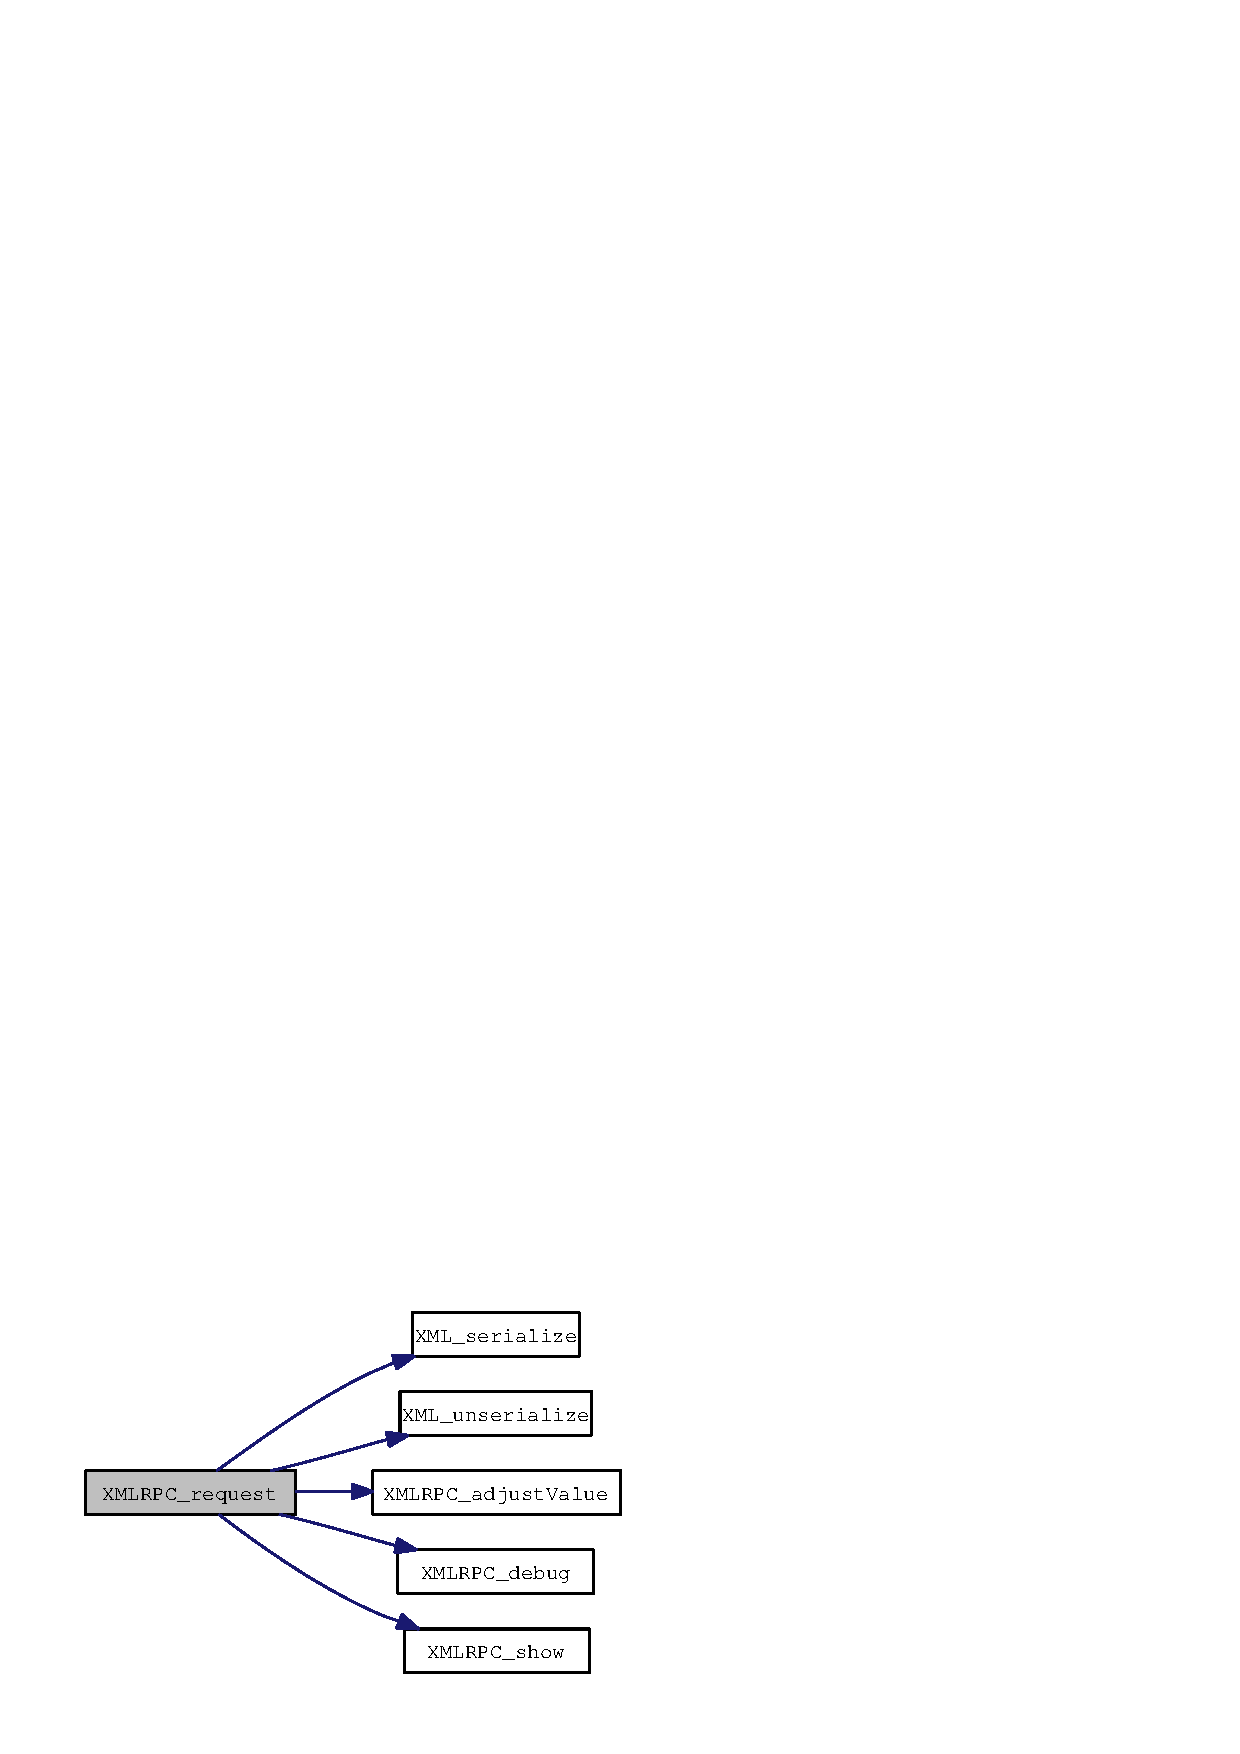
\includegraphics[width=151pt]{xmlrpc_8inc_3a98b6984b8ca01752d1aa9a267526a3_cgraph}
\end{center}
\end{figure}
\hypertarget{xmlrpc_8inc_c736d378caaccdd0726ea1080d1f526f}{
\index{xmlrpc.inc@{xmlrpc.inc}!XMLRPC_response@{XMLRPC\_\-response}}
\index{XMLRPC_response@{XMLRPC\_\-response}!xmlrpc.inc@{xmlrpc.inc}}
\subsubsection{\setlength{\rightskip}{0pt plus 5cm}XMLRPC\_\-response (\$ {\em return\_\-value}, \$ {\em server} = {\tt NULL})}}
\label{xmlrpc_8inc_c736d378caaccdd0726ea1080d1f526f}




Definition at line 418 of file xmlrpc.inc.

References XML\_\-serialize(), XMLRPC\_\-debug(), and XMLRPC\_\-show().

\begin{Code}\begin{verbatim}418                                                        {
419   $data["methodResponse"]["params"]["param"]["value"] = &$return_value;
420   $return = XML_serialize(&$data);
421 
422   if(defined('XMLRPC_DEBUG') and XMLRPC_DEBUG){
423     XMLRPC_debug('XMLRPC_response', "<p>Received the following data to return:</p>\n\n" . XMLRPC_show($return_value, 'print_r', true));
424   }
425 
426   header("Connection: close");
427   header("Content-Length: " . strlen($return));
428   header("Content-Type: text/xml");
429   header("Date: " . date("r"));
430   if($server){
431     header("Server: $server");
432   }
433 
434   if(defined('XMLRPC_DEBUG') and XMLRPC_DEBUG){
435     XMLRPC_debug('XMLRPC_response', "<p>Sent the following response:</p>\n\n" . XMLRPC_show($return, 'print_r', true));
436   }
437   echo $return;
438 }
\end{verbatim}
\end{Code}




Here is the call graph for this function:\nopagebreak
\begin{figure}[H]
\begin{center}
\leavevmode
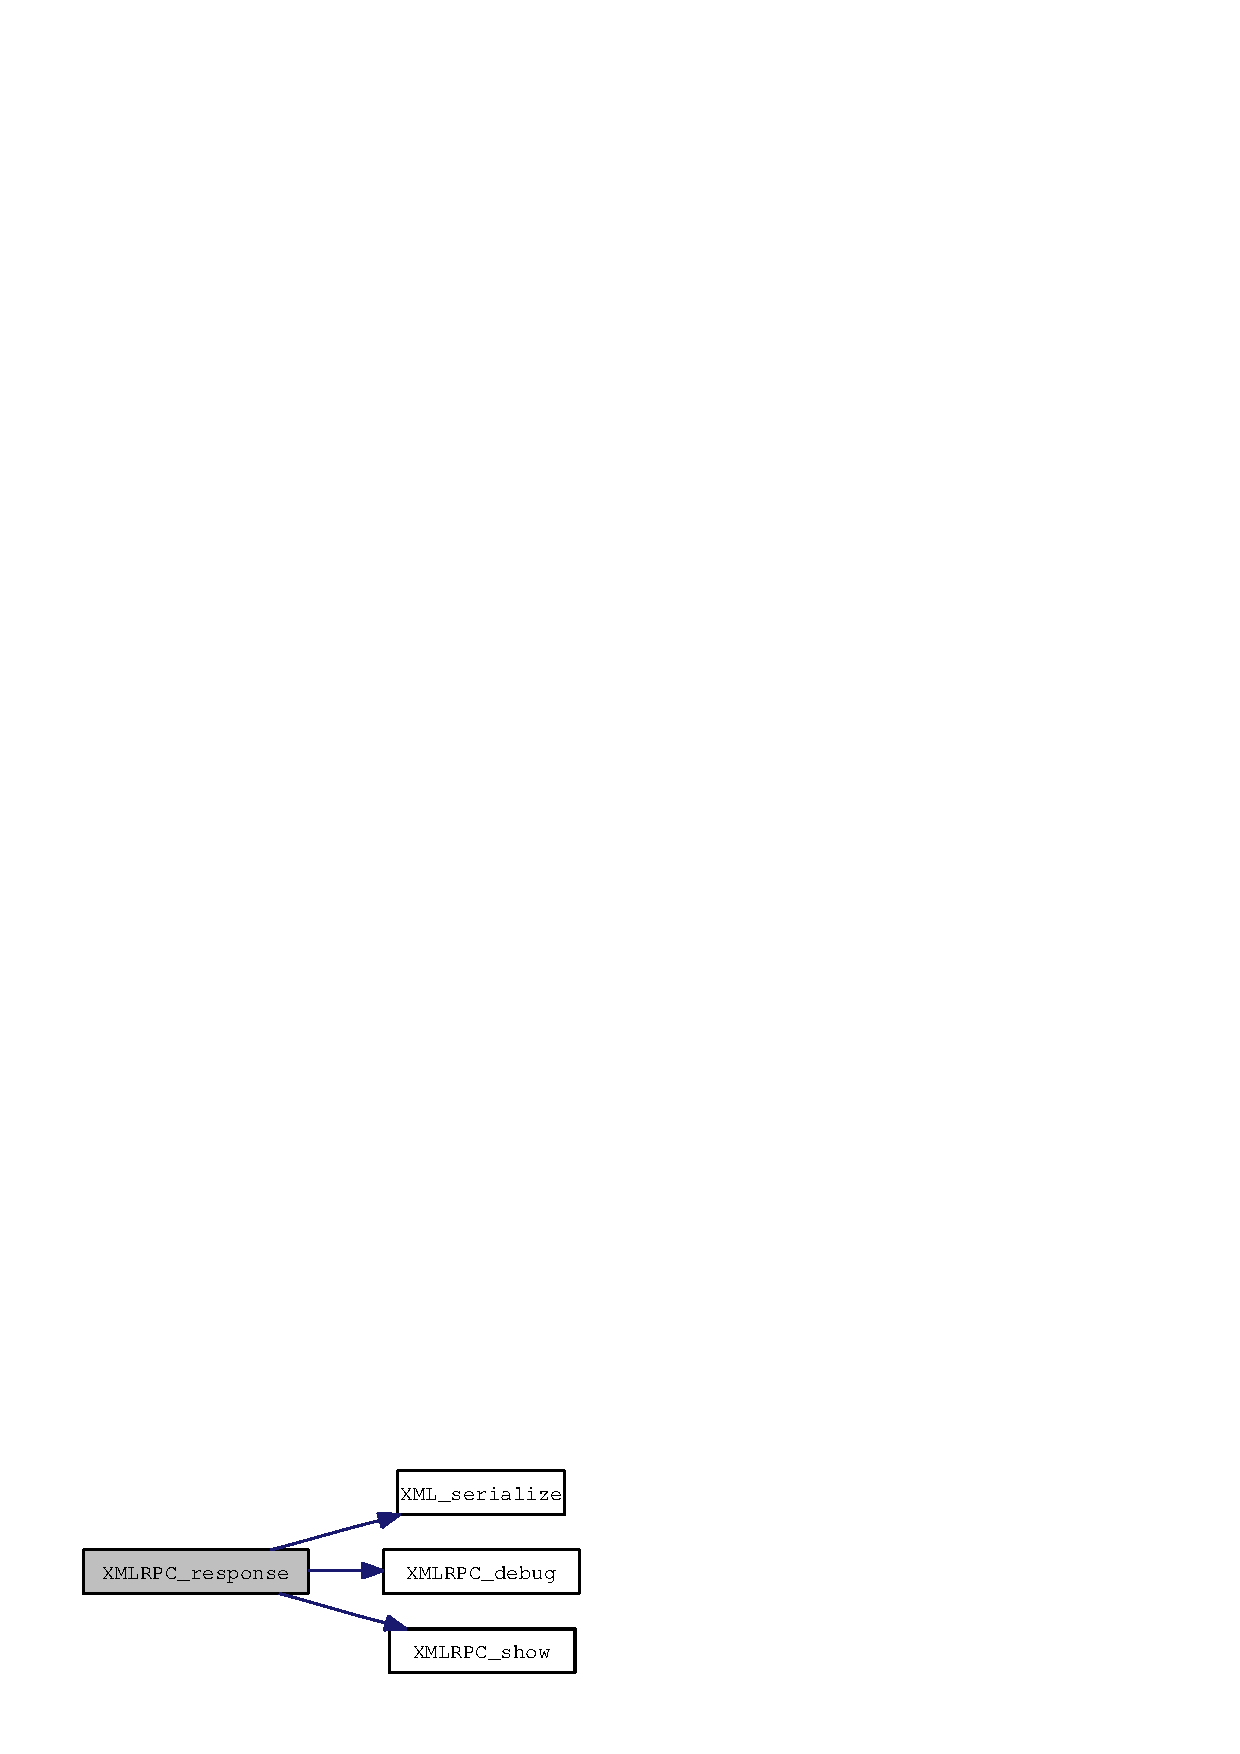
\includegraphics[width=141pt]{xmlrpc_8inc_c736d378caaccdd0726ea1080d1f526f_cgraph}
\end{center}
\end{figure}
\hypertarget{xmlrpc_8inc_1f60d2672bcb35f5ff908f64931f8d48}{
\index{xmlrpc.inc@{xmlrpc.inc}!XMLRPC_show@{XMLRPC\_\-show}}
\index{XMLRPC_show@{XMLRPC\_\-show}!xmlrpc.inc@{xmlrpc.inc}}
\subsubsection{\setlength{\rightskip}{0pt plus 5cm}XMLRPC\_\-show (\$ {\em data}, \$ {\em func} = {\tt \char`\"{}print\_\-r\char`\"{}}, \$ {\em return\_\-str} = {\tt false})}}
\label{xmlrpc_8inc_1f60d2672bcb35f5ff908f64931f8d48}




Definition at line 494 of file xmlrpc.inc.

Referenced by XMLRPC\_\-error(), XMLRPC\_\-parse(), XMLRPC\_\-request(), and XMLRPC\_\-response().

\begin{Code}\begin{verbatim}494                                                                    {
495   ob_start();
496   $func($data);
497   $output = ob_get_contents();
498   ob_end_clean();
499   if($return_str){
500     return "<pre>" . htmlspecialchars($output) . "</pre>\n";
501   }else{
502     echo "<pre>", htmlspecialchars($output), "</pre>\n";
503   }
504 }
\end{verbatim}
\end{Code}


